\documentclass{article}

\usepackage[utf8]{inputenc} % Required
\usepackage{lettrine} % Make first letter large
\usepackage[base]{babel} % Proper Latin hyphens
\usepackage{fontspec} % Use custom fonts
\usepackage{lipsum} % Generate Random Text (Lorem Ipsum)
\usepackage[a4paper, total={6in, 8in}]{geometry} % Change format to A4
\usepackage{multicol} % Three Columns (SN wants that)
\usepackage{fancyhdr} % Header
\usepackage[dvipsnames]{xcolor} % Many colors (Many)
\usepackage{lmodern}
\usepackage[T1]{fontenc} % Better Font Encoding
\usepackage{graphicx} % Graphics Rendering
\usepackage{caption}
\usepackage{gensymb}
\usepackage{float}

\graphicspath{ {./img/} } % Set Graphics Path
\DeclareGraphicsExtensions{.png,.pdf} % Do not allow JPGs


\newcommand*{\captionsource}[2]{%
    \caption*{%
        \noindent%
        {\fontsize{8pt}{8pt}%
            \selectfont \noindent \null \hfill \emph{#2}%
        }%
        \\\hspace{\linewidth}%
        {\fontsize{10pt}{10pt}%
            \selectfont \noindent \centering{#1}%
        }%
    }%
}


% The color SN uses for
% the header
\definecolor{SNBlue}{HTML}{005AAF} % Whoever decided to call HEX color codes HTML Color Codes should be tried for murder

% Customizing the header
\pagestyle{fancy}
\fancyhf{}
\fancyhead[R]{\textbf{Dec. 8, 2021}}
\fancyhead[L]{\textbf{Page 4}}
\fancyhead[C]{\textbf{\color{SNBlue}{SPACEPORT NEWS}}}

% Thicccer header
\renewcommand{\headrulewidth}{1pt}
% Set Header Color
\renewcommand{\headrule}{{%
    \color{SNBlue}\hrule height \headrulewidth\hfill}
}

\title{MarsAnalysis}
\date{December 2021}

% Font
\setmainfont[
    Path=fonts/,
    BoldItalicFont=Carlito-BoldItalic.ttf,
    BoldFont=Carlito-Bold.ttf,
    ItalicFont=Carlito-Italic.ttf,
    SizeFeatures={Size=11}
]{Carlito-Regular.ttf} % Set Font
% Document

\begin{document}

{
    \noindent
    \begin{center}
        \topskip0pt
        \vspace*{\fill}
        This is the result of having too much leisure time on one weekend.\\
        The first page was styled to look like the original space-port magazine from 2014 (minus the font). The new ones are ugly. \\
        (Also a result of too much leisure time).\\
        Don't be shocked about the page count, there are a \textbf{lot} of images.\\
        This is a PDF so that words cannot be counted. \\
        Topic was the landing spot on Mars.
        \vspace*{\fill}
    \end{center}
}
\pagebreak


% Title
\noindent
{\fontsize{40pt}{42pt}
    \selectfont \noindent \textbf{The Red Quest: A Journey into the unknown. But where to?}
}

\vspace{\baselineskip} % Prettier line

% Author + Date
\noindent % No Annoying Space at start of paragraph
\textbf{\emph{By Clemens Schütz}} % TextBF = Bold, Emph = Italic

\noindent % same here
\emph{Spaceport News}


\begin{multicols}{3}% Start layout

\noindent
\lettrine[lraise=0.1, nindent=0em, slope=-.5em]{\textbf{H}}{umanities} need
to explore that unbeknownst to it is as old as
the human thyself. 
\noindent
No matter what was discovered and uncovered, the human yearned for more - For better, or for worse. 
It comes to no suprise, that since the day that humanity has learned about what lies beyond
the blue tint of our sky, it has longed to
explore it.
And we have managed to do so well.
We have reconnoitred the hills of the moon
which seems to be so afar just 63 years ago - A Timespan that while seeming lingering is truly insignificant in the long history of human exploration.
After fulfilling this long-standing wish of humanity, it
would have been uncustomary, unnatural even, for humanity to be satisfied.
It set it's eyes on it's next target. Our Red Neighbour.
Yet still, 5 duodecennials after mankind has not been able to land a human being on our neighbour.
Even though it may seem as if little has progressed, this seems so only at first glance.
At second glance, one realizes just how much we have progressed.
If the quest to land a human on Mars was a race, we would be approaching the finish line at exponential speed.
Still, a plethora of issues must still be adressed, questions must be answered and math must be solved. % Look at this again
\\ % Newline
One of said questions is the long-standing question of where to land.
Some consider this a question easily solved, but this also seems so only at first glance - Just like so many problems in the world of aerospace engineering.
If a group of 100 scientists, each of them in different fields, was asked the question asked above, responses would diverge from each other massively. 
This is why the will of scientists must not influence the ultimate landing spot.
Additionally, space agencies should first contrive to land a human on Mars before making promises to researchers.
The above reasons contribute to the idea that the ideal landing spot should be decided through data.
As good maps are as scarce as billionaires with a working moral compass, the result of this should not be considered as good.
\\
The following part consists of two analysis. Both times different maps that represent different factors were used.
This was necessary as NASA does not seem capable of deciding what format of map they like more.
After that, these results are compared with those of another research paper as well as those of NASAs official blog.

\section{The Concept}

Viewed abstractly, the concept seems simple.
All Maps are being read pixel by pixel and stored as an one-dimensional array of colors.
Then the first array shall be iterated over, comparing itself indexed by the iterative position at \(colors\_of\_first\_image[i]\).
Let \(i\) be a variable which is incremented each iteration and let the operator \([i]\) return the element of the array at position \(i\).
If all Colors are equal at said position, the pixel and its color are stored and drawn on a grayscale-version of the image

In practice, it is as simple as it seems, as soon as one problem is overcome.
NASA seems to be incapable of deciding on one color-palette for all of their maps.
Therefore, each color must be matched with one of fourteen major colors.
This is, luckily, very easy.
In color science, a concept of color space exists, in which all RGB colors can be found.
In said space, a distance that one color has from another can be calculated using euclidean geometry very easily and is defined as the following.

\end{multicols}
\begin{figure}[H]
\[distance = \sqrt{(R_2 - R_1)^2 + (G_2 - G_1)^2 + (B_2 - B_1)^2}\]
\caption{Euclidean distance in color space}
\end{figure}
\begin{multicols}{3}
In this context \(*_2\) is either the red \(R\), green \(G\) or blue \(B\) factor of \(Color 2\).
For \(*_1\) the same applies, just for \(Color 1\). 
Then, the distances from all major colors is calculated and the nearest is taken.
This, unfortunately, makes slight differences in colors useless.
It would make it way harder to detect said differences, which is why I decided to ignore them. The data analysis was meant to be easy to make, not exact.

\section{The First Analysis}
In this analysis a total of four maps were used.

\end{multicols}
\begin{figure}[H]
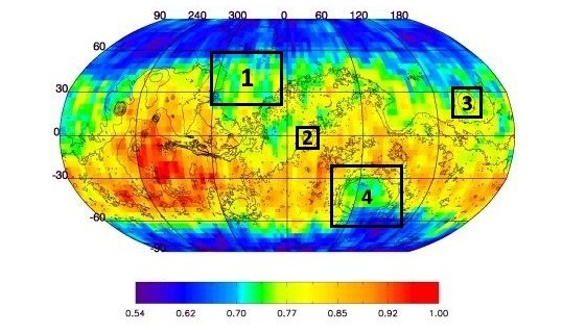
\includegraphics[width=\textwidth]{first/raw/neutron_rad.jpg}
\captionsource{Neutron Radiation on Mars surface}{NASA/JPL}
\label{fig:neutron_rad}
\end{figure}
\begin{multicols}{3}

\end{multicols}
\begin{figure}[H]
\noindent\makebox[\textwidth]{
    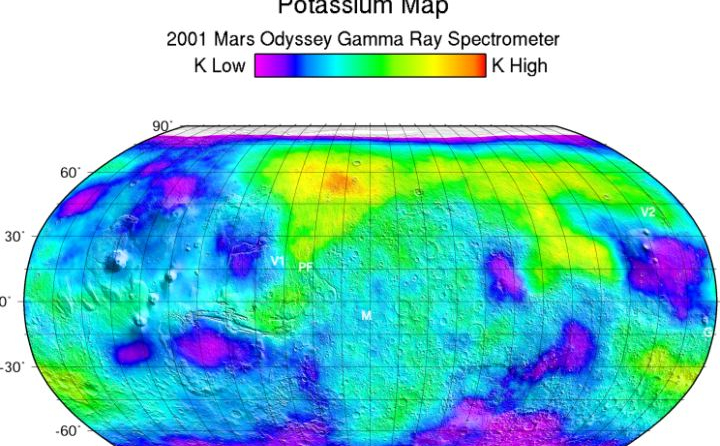
\includegraphics[width=\textwidth]{first/raw/radiation.png}
}
\captionsource{Potassium on Mars surface}{NASA/JPL}
\label{fig:raditation}
\end{figure}
\begin{multicols}{3}


\end{multicols}
\begin{figure}[H]
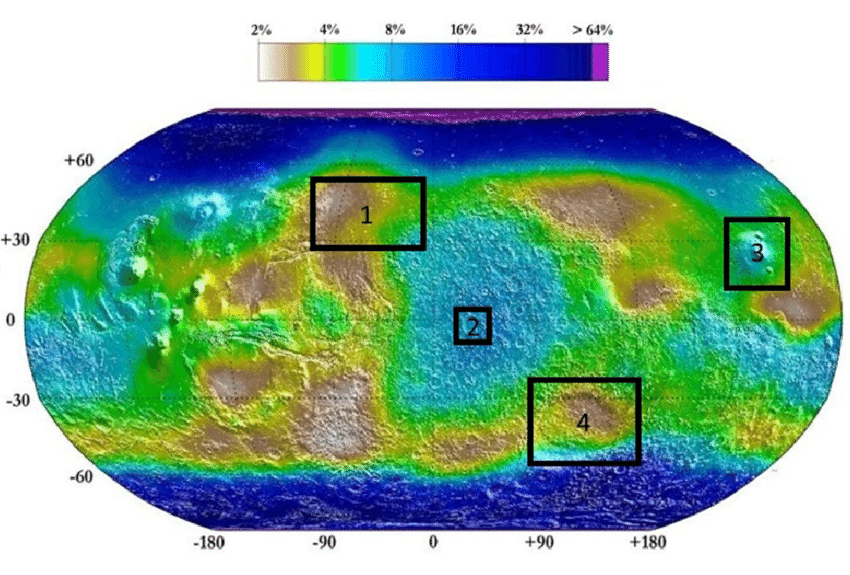
\includegraphics[scale=0.5, width=\textwidth]{first/raw/waterice.png}
\captionsource{Water content on the surface of Mars}{NASA/JPL}
\label{fig:waterice}
\end{figure}
\begin{multicols}{3}


\end{multicols}
\begin{figure}[H]
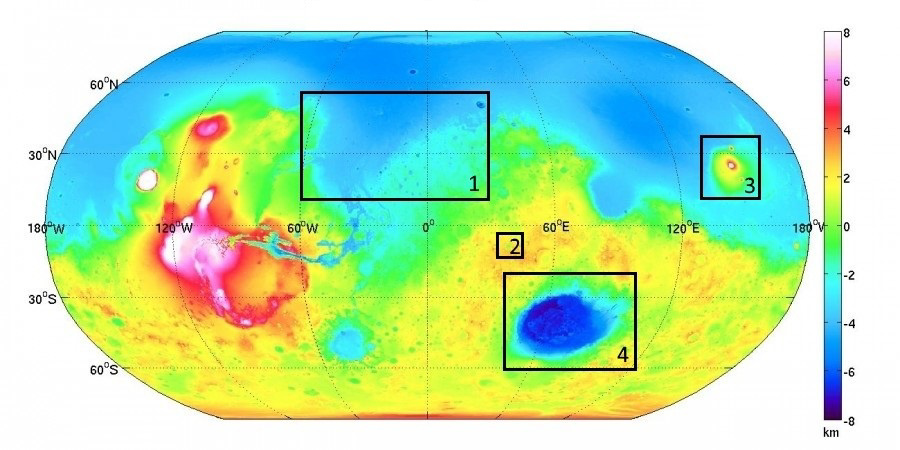
\includegraphics[scale=0.5, width=\textwidth]{first/raw/topography.jpg}
\captionsource{Mars's topography}{https://asu.cas.cz}
\label{fig:topography}
\end{figure}

The following map visualizes all of the maps that have a color in common.

\begin{figure}[H]
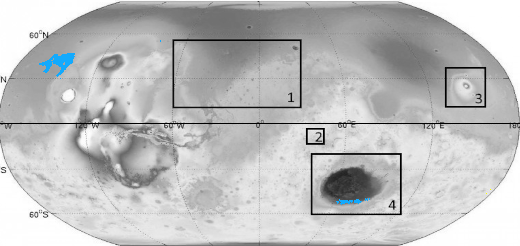
\includegraphics[scale=0.5, width=\textwidth]{first/out/out.first.downscaled.png}
\captionsource{The End Result of the first analysis}{/}
\label{fig:result1}
\end{figure}

As seen, there is only a small amount of pixels which are the same on all images.
In total, only \(470\) pixels overlap.
Interesting is, that all of the overlaps seem to be of the major color \(LightBlue\).
This may be explained with the fact that \(LightBlue\) represents a moderate value with a tendency to being good.
Therefore, this is a very good result.

\begin{figure}[H]
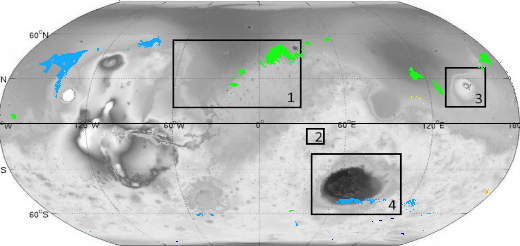
\includegraphics[scale=0.5, width=\textwidth]{first/out/out.first.downscaled.without_topo.png}
\captionsource{The End Result of the first analysis \textbf{without topography}}{/}
\label{fig:endres_wt}
\end{figure}

If we remove the map showing topography, we get a much more promising result.
Without topography, a total amount of \(1725\) pixels are yielded, which fulfill the requirement of having the same colour in all images.

Using this map, we can identify a total of four zones that may be good landing spots.
The following data is \textbf{slightly} unreliable. As the maps had \textbf{slightly} different scales, a margin of error of about \(\pm 10 \degree\) in both directions exists.
\begin{enumerate}
\item The first one is found around \(45 \degree N (latitude)\) and \(160 \degree W (longitude) \)
\item The second spot resides around \(45 \degree N (latitude)\) and \(20 \degree E (longitude)\)
\item The third spot may be seen at about \(30 \degree N (latitude)\) and \(120 \degree E (longitude)\)
\item The last spot is found at about \(45 \degree S (latitude)\) and \(60 \degree E (longitude)\)
\end{enumerate}

\section{The second analysis}
Temperature may not be forgotten about entirely.
Temperatures on Mars are harsh ranging from \(-120 \degree\) by night to \(20 \degree\) by day.
As the temperatures diverge so drastically, two maps, one for day and one for the night, must be used.
The following maps were used.

\begin{figure}[H]
    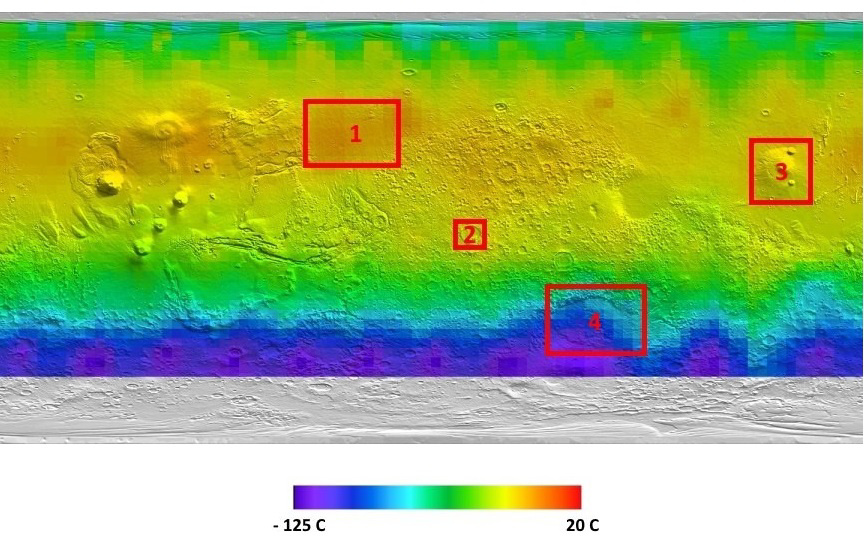
\includegraphics[scale=0.5, width=\textwidth]{second/raw//daytime.jpg}
    \captionsource{Temperature by day on Mars}{NASA/JPL}
    \label{fig:tempbyday}
\end{figure}

\begin{figure}[H]
    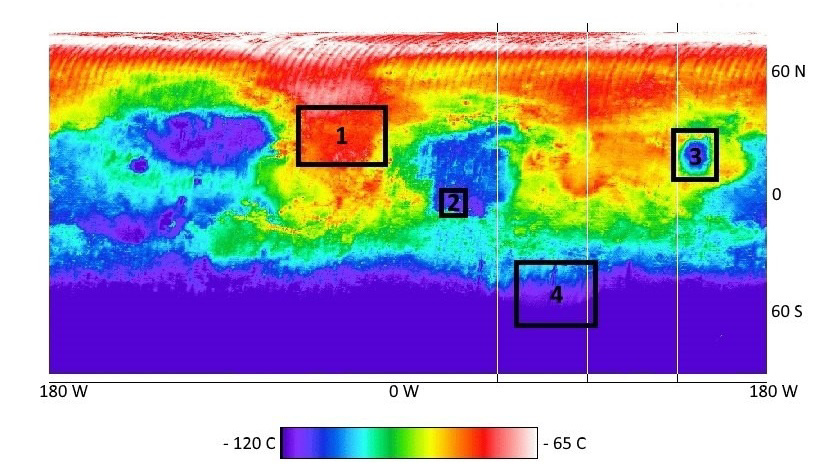
\includegraphics[scale=0.5, width=\textwidth]{second/raw/nighttime.jpg}
    \captionsource{Temperature by night on Mars}{NASA/JPL}
    \label{fig:tempbynight}
\end{figure}
If we repeat the above-mentioned process here, the following map is yielded. 

\begin{figure}[H]
    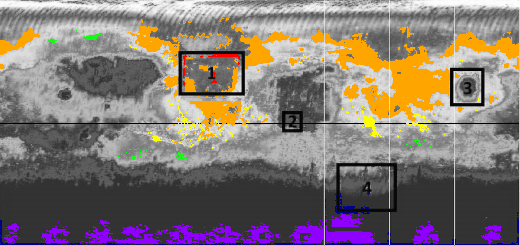
\includegraphics[scale=0.5, width=\textwidth]{second/out/out.second.downscaled.png}
    \captionsource{The End result of the second analysis}{NASA/JPL}
    \label{fig:tempend}
\end{figure}

As seen here, two areas of optimal climate were identified.
\begin{enumerate}
\item The first area is between \(0 \degree N (latitude)\) and  \(60 \degree N(latitude) \) latitude and \(45 \degree W(longitude)\) and \(0 \degree W (longitude)\) longitude.
\item The second area resides between \(0 \degree N (latitude)\) and \(60 \degree N (latitude) \) latitude and \(80 \degree E (longitude) \) and \(135 \degree E (longitude) \) longitude.
\end{enumerate}
Now, we are able to compare the four points mentioned above with this map in order to find the temperatures at this point.

\subsection{The First Point}
The first point is somewhere around \(45 \degree N (latitude)\) and \(160 \degree W (longitude) \). \\
While being within the latitude requirements (\(\pm 0 \leq lat \leq +60 \;|\; \pm 0 \leq lat \leq +60,\; lat = +45 N\)), it is outside of the longitude requirements (\(  \pm 0 \leq long \leq +45 \;|\; -80 \leq long \leq -135,\; long = +160 \))
This spot should not be considered as the primary landing spot.

\subsection{The Second Spot}
The second spot may be found around \(45 \degree N (latitude)\) and \(20 \degree E (longitude)\). \\
While being within the latitude requirements (\(\pm 0 \leq lat \leq +60 \;|\; \pm 0 \leq lat \leq +60,\; lat = +45 N\)), it is just slightly outside of the longitude requirements (\(  \pm 0 \leq long \leq +45 \;|\; -80 \leq long \leq -135,\; long = -20 \))
This spot is, sadly, not a good landing spot.

\subsection{The Third Spot}
This spot's coordinates are somewhere around \(30 \degree N (latitude)\) and \(120 \degree E (longitude)\). \\
It fulfills both the latitudes (\(\pm 0 \leq lat \leq +60 \;|\; \pm 0 \leq lat \leq +60,\; lat = +30 N\)), as well as the longitude requirements (\(  \pm 0 \leq long \leq +45 \;|\; -80 \leq long \leq -135,\; long = +20 \)).
Therefore, this spot would be a good landing spot.

\subsection{The Fourth Spot}
The fourth spot is found around \(45 \degree S (latitude)\) and \(60 \degree E (longitude)\). \\
It does not fulfill the latitudes requirements (\(\pm 0 \leq lat \leq +60 \;|\; \pm 0 \leq lat \leq -60,\; lat = +45 N\)), while still fulfilling the longitudes (\(  \pm 0 \leq long \leq +45 \;|\; -80 \leq long \leq -135,\; long = -60 \)).
This spot also fails to meet the requirements

\section{Conclusion}
Only one spot was able to reach all of the requirements, while still being within
This spot is found around \(25 \degree N (latitude)\) and \(120 \degree E (longitude)\), but, as of the margin of error, the ideal spot may be located closer to \(30 \degree N (latitude)\) and \(150 \degree E (longitude)\)  \\
Said spot is an ideal landing spot due to a huge amount of reasons.
\begin{enumerate}
    \item The neutron radiation has a factor of about \(0.75\). \\
    \item Potassium radiation was not detected in huge masses.
    \item It's altitude ranges from \(0km\) to \(12km\) at the peak.
    \item The water content is about \(10\%\).
    \item It's daytime-temperatures are about \(-10 \degree C\)
    \item It's nighttime-temperatures range from \(~-55 \degree C\) down to \(~-100 \degree\) depending on altitude. 
    \item The spot is exactly where the Elysium Mons is located
\end{enumerate}

Even though it was said before that researchers should be ignored, they should be happy about this place due to the attributes of the Elysium Mons.

\subsection{The Elysium Mons}
As mentioned before, the ideal landing spot is around the Elysium Mons.
This Mountain does not only have a great name, but also a few interesting attributes.
\begin{enumerate}
    \item It's peak is \(12.6km\) high.
    \item A crater with a diameter of \(6.5\) kilometers was found just next to the mountain \(29.674N, \; 130.799E\). \\ Therefore, lower layers of the mars may be viewed.
\end{enumerate}

During the astronauts two-year stay on Mars, volcanic activity can be studied, as the Elysium Mons was a volcano once.
\\
Additionally, Nakhlite Meteorites may be studied. 
Those are martian meteorites with an age of about \(10.7 Ma\).
This suggests that all of these meteorites were ejected by single impact event.
The differentiating ages of those meteorites plus the crater dimensions suggest a growth rate of the source volcano which is far slower than the expected one.
This implies that the martian volcanic activity has slowed down greatly by the impact event.

Additionally, a similar conclusion was reached in the paper "GIS analysis of promising landing sites for manned flight to Mars", which lists the Elysium Mons as one of four possible landing locations. \cite{dmtri}


\begin{thebibliography}{1}
    \bibitem{dmtri}
    Kuziakina, M., Gura, D. and Zverok, D., 2019. GIS analysis of promising landing sites for manned flight to Mars. E3S Web of Conferences, 138, p.02004.
\end{thebibliography}
    
\end{document}
